\documentclass[11pt,a4paper]{article}
\usepackage[T1]{fontenc}
\usepackage[margin=2.3cm]{geometry}
\usepackage{amsmath,amssymb}
\usepackage{graphicx}
\usepackage[dvipsnames]{xcolor}
\usepackage{enumitem}
\usepackage[colorlinks=true,linkcolor=blue,urlcolor=blue]{hyperref}
\setlength{\parskip}{0.6em}
\setlength{\parindent}{0pt}
\begin{document}

\begin{center}{\LARGE\bfseries openpacket}\\[0.4em]{\large Follow a packet across the internet, from browser to server, in three sessions.}\\[0.2em]\small PAN IIT OSS explainer \textbullet{} secondary school to diploma / undergraduate (levels 3-5)\end{center}

\section*{Why this exists}
Every web page you open is cut into packets that cross many routers. This explainer shows the mathematics behind that journey: addresses as numbers, routing by longest prefix, the delay budget and a tiny simulator you can run on your own computer.

\section*{The end goal}
Follow a packet across the internet from browser to server. The end goal is to follow a packet across the internet from browser to server: what is in it, how each router chooses where it goes, how long it takes, and what happens when queues fill or links fail. The same ideas lie behind video calls, cloud services and mobile networks.

\section*{How the three sessions build up}
\begin{enumerate}[nosep]
\item \textbf{Session 1: A message is cut into packets that hop from router to router} (Level 1, conceptual interactive model, 60 min).
\item \textbf{Session 2: The mathematics of a packet: headers, addresses, routing tables and delay} (Level 2, mathematical engineering model, 75 min).
\item \textbf{Session 3: A tiny network simulator: queues, loss, failures and validation} (Level 3, simulation and validation, 90 min).
\end{enumerate}

\section{Session 1: A message is cut into packets that hop from router to router}

\subsection*{A. Real-world problem}
When you open a web page the server does not send it in one piece. The page is cut into many small packets. Each packet is labelled with where it is going and which piece it is, and routers pass it on from one to the next, like post offices passing a parcel. Why not send the whole page in one go? And how small should the pieces be? (This is a simplified educational model of the internet.)

\subsection*{B. Concept and theory}
A message of M bytes is cut into packets of at most s bytes of payload, so the number of packets is N = ceil(M / s): round up, because the last packet may be shorter. Every packet also carries a label (header) of h bytes with the addresses and the sequence number; here h = 40 bytes. Each router knows only the next hop for each destination, never the whole path. A link carries one packet at a time and a router can pass a packet on only after receiving all of it (store and forward). Let one step be the time one packet needs to cross one link. The first packet needs H steps for H hops and every other packet arrives one step after the one before it, so the whole message needs H + N - 1 steps. One step lasts (s + h) * 8 / R seconds on a link of R bit/s, which gives the delivery time.

\begin{itemize}[nosep]
\item M: message size (bytes)
\item s: payload per packet (bytes)
\item h: label (header) per packet, 40 here (bytes)
\item N: number of packets (no unit)
\item H: number of hops (links) on the route (no unit)
\item R: link rate, 1 000 000 here (bit/s)
\item T: delivery time of the whole message (s or ms)
\end{itemize}

\begin{equation*}
N=\left\lceil \frac{M}{s}\right\rceil
\end{equation*}

\begin{equation*}
\text{steps}=H+N-1
\end{equation*}

\begin{equation*}
T=(H+N-1)\,\frac{8\,(s+h)}{R}
\end{equation*}

\begin{center}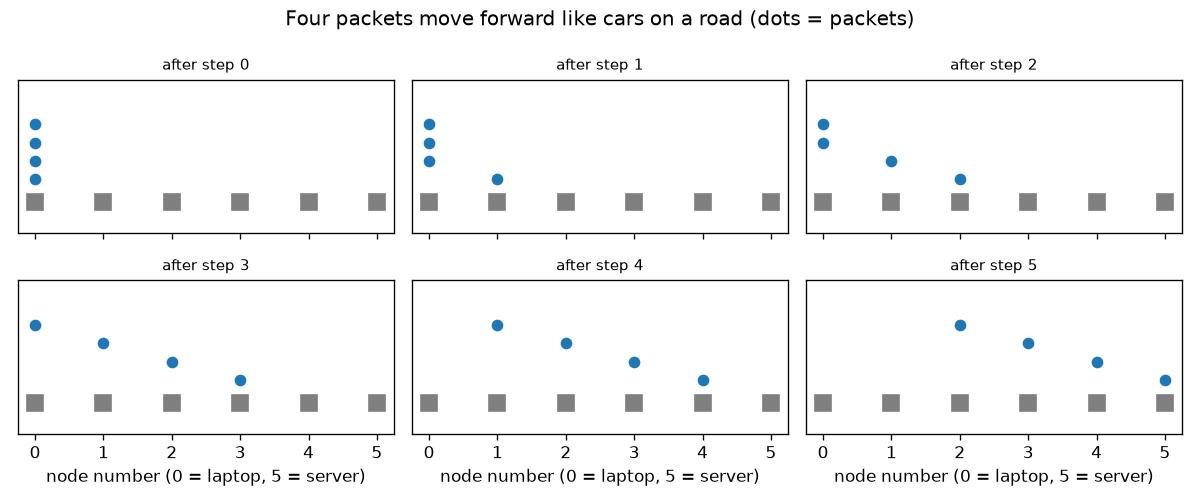
\includegraphics[width=0.85\linewidth]{figures/s01_packet_journey.png}\\\small Four packets crossing five hops, one picture per step: they follow each other like cars on a road.\end{center}

\subsection*{E. Worked example}
A 1000 byte message is sent in packets of 300 bytes of payload over 3 hops. Links run at 1 Mbit/s and every packet has a 40 byte label. How many packets are there, how many steps, and how long does the delivery take?
\begin{enumerate}[nosep]
\item N = ceil(1000 / 300) = ceil(3.33) = 4 packets (300, 300, 300 and 100 bytes).
\item Steps = H + N - 1 = 3 + 4 - 1 = 6.
\item One step = (300 + 40) * 8 / 1 000 000 = 0.00272 s = 2.72 ms.
\item T = 6 * 2.72 ms = 16.32 ms.
\item Check by simulation: journey\_steps(4, 3) moves the packets one step at a time and also gives 6.
\end{enumerate}
\textbf{Answer.} 4 packets, 6 steps and 16.32 ms.

\subsection*{F. Questions}
\begin{enumerate}[nosep]
\item \textbf{Conceptual.} Why does every packet carry a sequence number? What goes wrong without it?
\item \textbf{Numerical.} A 900 byte message is sent in packets of 250 bytes of payload over 4 hops at 1 Mbit/s, with a 40 byte label per packet. Find the number of packets, their sizes, the steps and the delivery time.
\item \textbf{Graph and simulation interpretation.} In the graph of delivery time against payload size (1000 byte message, 5 hops), the time is 25.92 ms for 20 byte packets, 15.68 ms for 100 byte packets and 41.6 ms for one 1000 byte packet. Explain the shape of the curve.
\item \textbf{Design and optimisation challenge.} Design: for the 1000 byte message over 5 hops, compare payloads of 50, 100, 200 and 500 bytes and choose one. What would make you choose a larger size in real life?
\end{enumerate}

\section{Session 2: The mathematics of a packet: headers, addresses, routing tables and delay}

\subsection*{A. Real-world problem}
A packet must say who sent it, where it is going, which piece of the message it is, and carry a check so that damage can be noticed. That costs bytes. Then every router must choose the next hop for it within a tiny fraction of a second, and the trip takes time that no technology can shrink below the speed of light in fibre. How large is the header overhead? How does a router choose? How fast can a packet get from Delhi to London? (Simplified educational model: the toy header is not the real IPv4 header.)

\subsection*{B. Concept and theory}
An IPv4 address is four bytes, so it is a 32-bit number: 192.168.1.20 is 192*256\textasciicircum{}3 + 168*256\textasciicircum{}2 + 1*256 + 20 = 3232235796. A subnet written 192.168.1.0/24 fixes the first 24 bits (the network) and leaves 8 bits for hosts, so it holds 2\textasciicircum{}8 = 256 addresses. The mask has 24 ones followed by zeros; an address is inside when (address AND mask) equals the network. A router table has rows (prefix, next hop); when several rows match, the router uses the one with the longest prefix, and 0.0.0.0/0 is the default route. A toy packet has a 14 byte header (source 4, destination 4, sequence 2, payload length 2, checksum 2) followed by the payload; the checksum adds all 16-bit words, folds the carries and flips the bits so that a receiver adding everything gets all ones. The one-way delay over a link is propagation (distance divided by the signal speed, about 2e8 m/s in fibre, two thirds of the speed of light in vacuum) plus transmission (bits divided by bandwidth) plus queueing. The smallest possible round trip is twice the distance divided by the signal speed. The header overhead for header h and payload p is h / (h + p), which is below a limit x when p \textgreater{} h (1 - x) / x.

\begin{itemize}[nosep]
\item a: IPv4 address as a number (no unit (0 to 2\textasciicircum{}32 - 1))
\item n: prefix length of a subnet (bits)
\item d: distance along the link (m)
\item v: signal speed in fibre, about 2e8 (m/s)
\item L: packet size in bits (bit)
\item B: link bandwidth (bit/s)
\item q: queueing delay (s)
\item h, p: header and payload size (bytes)
\item x: overhead limit (0.05) (no unit)
\end{itemize}

\begin{equation*}
a=a_1\,2^{24}+a_2\,2^{16}+a_3\,2^{8}+a_4
\end{equation*}

\begin{equation*}
\text{inside}\iff (a\ \&\ \text{mask}_n)=\text{network},\qquad \text{size}=2^{32-n}
\end{equation*}

\begin{equation*}
t_{\text{one-way}}=\frac{d}{v}+\frac{L}{B}+q,\qquad \text{RTT}_{\min}=\frac{2d}{v}
\end{equation*}

\begin{equation*}
\text{overhead}=\frac{h}{h+p}<x\iff p>\frac{h\,(1-x)}{x}
\end{equation*}

\begin{center}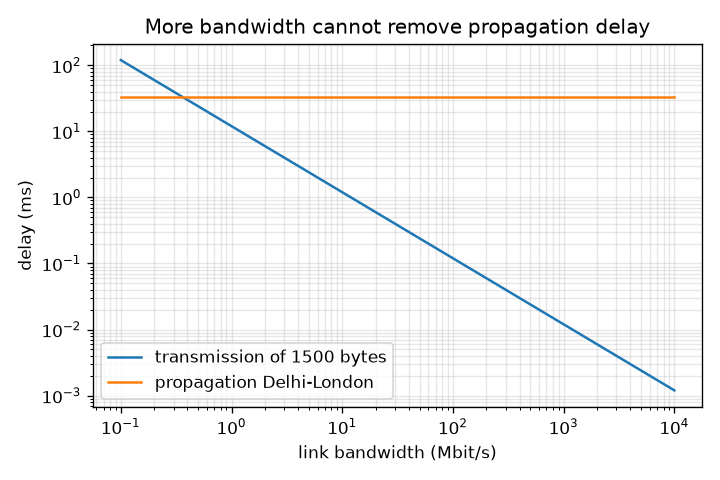
\includegraphics[width=0.85\linewidth]{figures/s02_delay_budget.png}\\\small Transmission delay of a 1500 byte packet against bandwidth, and the fixed Delhi to London propagation delay.\end{center}

\subsection*{E. Worked example}
A 1500 byte packet crosses Delhi to London (6712 km great-circle distance) on a 100 Mbit/s link and waits 2 ms in queues. Find the propagation, transmission and total one-way delay, and the minimum round-trip time.
\begin{enumerate}[nosep]
\item Propagation = d / v = 6.712e6 m / 2e8 m/s = 0.03356 s = 33.56 ms.
\item Transmission = L / B = (1500 * 8 bits) / 100e6 bit/s = 12000 / 1e8 = 0.00012 s = 0.12 ms.
\item Queueing = 2 ms (given).
\item Total one-way = 33.56 + 0.12 + 2 = 35.68 ms.
\item Minimum round trip = 2 d / v = 2 * 33.56 = 67.12 ms (no queueing, zero-size packet).
\end{enumerate}
\textbf{Answer.} Propagation 33.56 ms, transmission 0.12 ms, total one-way 35.68 ms, minimum round trip 67.12 ms.

\subsection*{F. Questions}
\begin{enumerate}[nosep]
\item \textbf{Conceptual.} Why must a router use the longest matching prefix rather than the first or shortest match? Give an example with the table in the lesson.
\item \textbf{Numerical.} How many addresses does a /20 subnet hold? Is 10.1.15.200 inside 10.1.0.0/20? Is 10.1.16.0?
\item \textbf{Graph and simulation interpretation.} In the overhead graph, at about what payload do the toy header (14 bytes) and the 40 byte header cross the 5 percent line? What does a flat tail of the curve tell you?
\item \textbf{Design and optimisation challenge.} Design: the header is 40 bytes, the link is 1 Mbit/s and the transmission time of one packet must not exceed 10 ms. Overhead must be below 5 percent. Which payload sizes are allowed? Which would you choose?
\end{enumerate}

\section{Session 3: A tiny network simulator: queues, loss, failures and validation}

\subsection*{A. Real-world problem}
Real networks are too big and too fast to watch, and you must not experiment on them. So we build a toy one inside the computer: routers are points on a graph, links have a delay and a bandwidth, and packets move hop by hop through queues. It uses no sockets and sends nothing anywhere, it is pure arithmetic. Can a simple simulator reproduce the delay formulas exactly? What happens when a buffer fills, a link is cut, or two routers send a packet in circles? (Simplified educational model, not a validated tool for designing real networks.)

\subsection*{B. Concept and theory}
Routing tables come from Dijkstra's algorithm: keep the cheapest known cost to every node, always expand the cheapest unexpanded node, and record for every destination the first hop. The simulator is event-driven: time jumps from event to event (a packet arrives, a transmission ends). Each directed link has a transmitter that sends one packet at a time (L/R seconds), a queue that holds at most B waiting packets (a packet that finds it full is dropped), and a wire delay d. A packet also has a time to live (TTL) that falls by one at every router, so a routing loop ends. A burst of n packets of size L sent at once into one link of rate R is delayed by k L/R plus d for the k-th packet, so queueing adds L/R for each packet ahead. With a finite buffer B, 1 + B packets of the burst get through and the rest are dropped. For reliable delivery a sender with window W sends W packets, waits for acknowledgements and resends after a timeout. With x = L/R and RTT the time from the end of sending a packet to the arrival of its acknowledgement, a window W uses the link a fraction U = min(1, W x / (x + RTT)) of the time; stop-and-wait is W = 1. If each transmission is lost with probability p, a packet needs 1/(1-p) transmissions on average. At every moment packets are conserved: sent = delivered + dropped + in flight. A toy congestion window (a simplified illustration, not real TCP) grows by 1 per round trip and halves when the pipe and buffer overflow; its average is about three quarters of its peak.

\begin{itemize}[nosep]
\item x = L/R: time to send one packet (s)
\item d: wire delay of a link (s)
\item B: buffer: packets allowed to wait (packets)
\item W: window: packets sent before waiting (packets)
\item RTT: time from end of sending to the acknowledgement arriving (s)
\item U: fraction of time the link is busy (no unit)
\item p: probability that a transmission is lost (no unit)
\item TTL: hops a packet may still make (no unit)
\end{itemize}

\begin{equation*}
D(v)=\min_{u}\big(D(u)+c(u,v)\big)\quad\text{(Dijkstra: cheapest cost to node }v\text{)}
\end{equation*}

\begin{equation*}
t_k=k\,\frac{L}{R}+d,\qquad k=1,2,\dots,1+B\quad\text{(burst into one link)}
\end{equation*}

\begin{equation*}
U=\min\!\left(1,\ \frac{W\,x}{x+\mathrm{RTT}}\right),\qquad x=\frac{L}{R}
\end{equation*}

\begin{equation*}
E[\text{transmissions}]=\frac{1}{1-p},\qquad \text{sent}=\text{delivered}+\text{dropped}+\text{in flight}
\end{equation*}

\begin{center}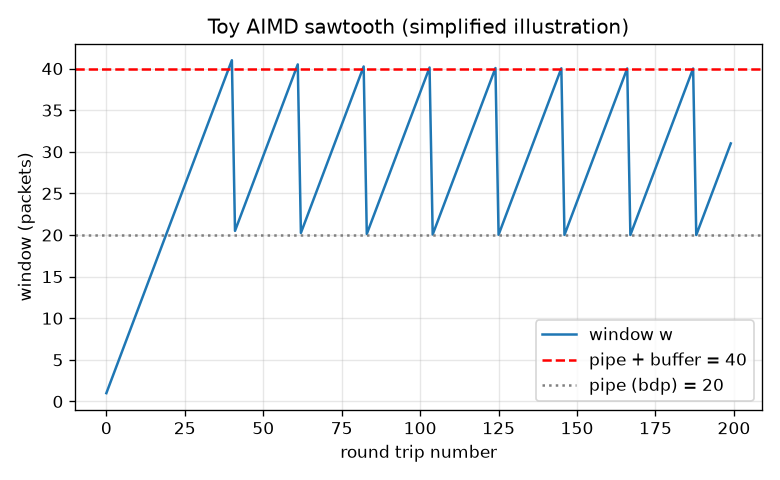
\includegraphics[width=0.85\linewidth]{figures/s03_aimd_sawtooth.png}\\\small Toy AIMD window (simplified illustration): sawtooth between about 20 and 40 packets.\end{center}

\subsection*{E. Worked example}
A burst of 10 packets of 1500 bytes (12000 bits) is sent at once into a link of 10 Mbit/s with 10 ms wire delay and a buffer of 4 waiting packets. How many arrive, how many are dropped, and what is the delay of the last one that arrives?
\begin{enumerate}[nosep]
\item Time to send one packet x = 12000 / 10e6 = 0.0012 s = 1.2 ms.
\item The first packet goes straight onto the wire; the next 4 wait in the buffer; the other 5 find it full and are dropped.
\item So 1 + 4 = 5 packets arrive, 5 are dropped.
\item The k-th packet finishes sending at k * 1.2 ms and arrives 10 ms later, so its delay is k * 1.2 + 10 ms.
\item The last one (k = 5) has delay 5 * 1.2 + 10 = 16.0 ms, of which queueing is 4 * 1.2 = 4.8 ms.
\end{enumerate}
\textbf{Answer.} 5 arrive and 5 are dropped; the last delivered packet has a delay of 16.0 ms, including 4.8 ms of queueing.

\subsection*{F. Questions}
\begin{enumerate}[nosep]
\item \textbf{Conceptual.} Why is stop-and-wait very inefficient on a link with a long delay, and what does a window change?
\item \textbf{Numerical.} A sender uses stop-and-wait with 1500 byte packets on a 10 Mbit/s link; the RTT after sending is 20.04 ms. Find x, U and the throughput. Which window fills the pipe?
\item \textbf{Graph and simulation interpretation.} In the re-routing graph, read the delay before the cut, after re-routing, and the number of lost packets. Why are exactly those packets lost, and how many would be lost if the failure were detected after 0.025 s instead of 0.05 s?
\item \textbf{Design and optimisation challenge.} Design: the router is upgraded from 16 to 20 buffer slots. A 20000 byte video frame is sent as one burst; each packet has a 40 byte header. What is the smallest payload that loses nothing now, and what happens with a payload of 761 bytes?
\end{enumerate}

\section{Real-world mini-project}
\textbf{Size the buffer and the packets for a video stream.} A camera sends 25 frames per second over one link of 5 Mbit/s with 10 ms delay. Each frame is 20000 bytes of payload that the camera cuts into packets (payload P bytes plus a 40 byte header) and sends all at once. The router at the other end of the link has memory for 16 waiting packets. Use \texttt{video\_trial} and \texttt{smallest\_payload} from Session 3 to find the smallest payload that loses nothing, check that the header overhead is below 5 percent, and check that no frame takes longer than 45 ms.

\section{The path ahead}
\begin{enumerate}[nosep]
\item \textbf{Session 4: Routers that talk to each other.} A routing protocol in the simulator where each router knows only its neighbours and exchanges tables, instead of the global Dijkstra.
\item \textbf{Session 5: Pace the video.} A paced sender for the video stream.
\item \textbf{Session 6: A sender that finds its own window.} A sender that starts with a window of 1 and adapts it to acknowledgements and losses.
\item \textbf{Session 7: Two senders share a link.} Two flows through the same router with the adaptive sender from the previous step.
\item \textbf{Session 8: Smarter queues.} A queue that drops early (for example random early detection) in place of tail drop.
\end{enumerate}

\section{Answers and hints}

\subsection*{Session 1}
\begin{enumerate}[nosep]
\item \textbf{Conceptual.} Hint: Packets may take different routes or queue for different times. Solution: Different packets can take different routes or wait in different queues, so they can arrive in a different order from the one in which they were sent. The sequence number lets the receiver sort them and rebuild the message; it also shows which packet is missing. Without it the receiver would have to trust the arrival order, and the page would be garbled.
\item \textbf{Numerical.} Hint: Round up for N; one step is (s + h) * 8 / R. Solution: N = ceil(900 / 250) = ceil(3.6) = 4 packets of 250, 250, 250 and 150 bytes. Steps = 4 + 4 - 1 = 7. One step = (250 + 40) * 8 / 1 000 000 = 2.32 ms, so T = 7 * 2.32 = 16.24 ms. (The last packet is shorter, so the real time is a little less; the model charges every packet full size.) Sanity check: the answer is close to the worked example, which has a similar size.
\item \textbf{Graph and simulation interpretation.} Hint: Two effects pull in opposite directions: the number of steps and the length of one step. Solution: With tiny packets there are many packets, so many steps, and a large share of every packet is label: 20 byte packets need 50 packets, 54 steps, each only 60 bytes long. With one huge packet there are only 5 steps but each one carries 1040 bytes and nothing overlaps, because only one link is busy at a time. In between, packets follow each other and the links work in parallel, and the curve has its lowest point near 100 bytes. The minimum is flat-ish: sizes near 100 are all good.
\item \textbf{Design and optimisation challenge.} Hint: Compute N, steps and T for each size. Solution: 50 bytes: 20 packets, 24 steps, 17.28 ms. 100 bytes: 10 packets, 14 steps, 15.68 ms. 200 bytes: 5 packets, 9 steps, 17.28 ms. 500 bytes: 2 packets, 6 steps, 25.92 ms. Best is 100 bytes. In real life routers also spend effort on every packet, so fewer packets save work, and real labels are a smaller share of a bigger packet; but a lost packet then costs more to resend. The trade-off is why real packets are about 1500 bytes, not 100.
\end{enumerate}

\subsection*{Session 2}
\begin{enumerate}[nosep]
\item \textbf{Conceptual.} Hint: A short prefix like 10.0.0.0/8 covers many addresses, including ones that have a more specific row. Solution: A longer prefix describes a smaller, more specific group of addresses, so it carries more precise information about where the address really is. 10.1.2.77 matches /0, /8, /16 and /24 rows; only the /24 row says it is in the lab, so the packet must go to the lab. If the router took the first or shortest match it would send it to the ISP or the corporate gateway, and the specific rows would never be used. The default route 0.0.0.0/0 is used only when nothing else matches.
\item \textbf{Numerical.} Hint: Size is 2 to the power (32 - 20). A /20 fixes the first 20 bits, so the third number is fixed in blocks of 16. Solution: Size = 2\textasciicircum{}(32 - 20) = 2\textasciicircum{}12 = 4096 addresses. The /20 covers 10.1.0.0 to 10.1.15.255 (the third number from 0 to 15). So 10.1.15.200 is inside, and 10.1.16.0 is just outside. Check: the mask is 255.255.240.0 and 15 AND 240 = 0, while 16 AND 240 = 16.
\item \textbf{Graph and simulation interpretation.} Hint: Solve h / (h + p) = 0.05 for p. Solution: p = h (1 - 0.05) / 0.05 = 19 h. For h = 14 that is 266 bytes (exactly 5 percent), so 267 bytes is the first whole number below the limit. For h = 40 it is 760 (exactly 5 percent), so 761 bytes is the first below. The tail is flat because adding payload to an already large packet saves very little overhead, while it makes each packet slower to send and costlier to resend.
\item \textbf{Design and optimisation challenge.} Hint: The overhead gives a minimum payload; the transmission limit gives a maximum: (p + 40) * 8 / 1e6 \textless{}= 0.010. Solution: Overhead: p \textgreater{}= 761 bytes. Transmission: p + 40 \textless{}= 10 ms * 1 Mbit/s / 8 = 1250 bytes, so p \textless{}= 1210 bytes. Allowed range: 761 to 1210 bytes. A choice near the upper end, such as 1000 bytes, keeps overhead low (3.85 percent) with some margin on the delay limit. The trade-off: larger packets have lower overhead but a lost packet costs more to resend and each packet blocks the link longer for others.
\end{enumerate}

\subsection*{Session 3}
\begin{enumerate}[nosep]
\item \textbf{Conceptual.} Hint: Think about how much of the time the sender is waiting for acknowledgements. Solution: In stop-and-wait the sender sends one packet and then waits for the acknowledgement, so most of each cycle is idle waiting; the link is busy only for x out of every x + RTT. A window lets the sender keep W packets in flight, so it fills the waiting time with more packets. The utilisation rises in proportion to W until the pipe is full. The price is more memory at the sender and more packets to resend when something is lost.
\item \textbf{Numerical.} Hint: x = L / R; U = x / (x + RTT); throughput = U * R. Solution: x = 12000 / 10e6 = 1.2 ms. U = 1.2 / (1.2 + 20.04) = 0.0565. Throughput = 0.0565 * 10 Mbit/s = 0.565 Mbit/s. The window that fills the pipe is the smallest W with W x \textgreater{}= x + RTT: W \textgreater{}= 21.24 / 1.2 = 17.7, so W = 18. Sanity check: U must be at most 1, and it is far below it, as expected for a long delay.
\item \textbf{Graph and simulation interpretation.} Hint: Packets are lost if they reach router R1 while its table still points at the broken link (and one is lost while being sent when the link breaks). Solution: Before the cut the delay is 18.6 ms (three links of 5 ms wire plus 1.2 ms sending each), after re-routing it is 33.6 ms (three links of 10 ms plus 1.2 ms each). 13 packets are lost: those that reach R1 from 1.2 ms before the cut until the tables are updated 0.05 s later, a window of about 51 ms with one packet every 4 ms. With a detection time of 0.025 s the window is about 26 ms and 7 packets are lost. The lost number is about the detection time divided by the packet interval, which is why fast failure detection matters.
\item \textbf{Design and optimisation challenge.} Hint: A frame of n packets needs n - 1 waiting slots. Find the smallest payload with n \textless{}= 21. Solution: With 20 slots the frame can have at most 21 packets: n = ceil(20000 / P) \textless{}= 21 needs P \textgreater{}= 953 (20000 / 21 = 952.4, so P = 953). Its overhead is 40 / 993 = 4.03 percent. With payload 761 there are 27 packets and 26 slots would be needed, so 6 packets of every frame are lost with 20 slots. Trade-off: smaller packets give a finer-grained loss but need more buffer for a burst; larger packets save header bytes but one loss destroys more data.
\end{enumerate}

\section{How to join}
Read \texttt{CONTRIBUTING.md} in the repository, then pick an issue labelled \texttt{good first issue}. Repository: \url{https://github.com/KrunalPanchal1995/openpacket}

\end{document}
